\lhead{\emph{Basic Operation}}

\chapter{Basic Operation}\label{ch:operation}

% In Chapter~\ref{ch:amcP}, the overall system has been described.  Each component of the system was discussed in detail.

% This chapter is about
% \begin{itemize}
%     \item how the system works as a unit to provide magnetic field control.  This includes the algorithm which generates the control and some typical results from its operation.  It also includes the methods used in operating the system, such as methods used in tuning the PI control system.
%     \item simulation methods used to understand system performance, and some basic results from the simulation which are compared with data
%     \item definition of metrics that will be used to quantify further system performance.  These will be applied in Chapter~\ref{ch:quantification} where further results will be presented.
% \end{itemize}



% Much of this work follows the work of others, especially Refs.~\cite{bea,rawlik,lins}.  New work that builds on these results is presented in Chapter~\ref{ch:quantification}.

%This chapter describes the main tool that generates the required currents that should be fed to the coils for compensation.
%The algorithm is based on the control theory and similar to as discussed in Ref. \cite{bea}.

In Chapter~\ref{ch:amcP}, the overall system has been described.  Each component of the system was discussed in detail. This chapter is about how the system works as a unit to provide magnetic field control.  This includes the algorithm which generates the control and some typical results from its operation.  It also includes the methods used in operating the system, such as methods used in tuning the control algorithm for the system. In addition to that, it will cover the simulation methods used to understand the system performance and some basic results from the simulation which are compared with the data. Finally, it will end with the definition of metrics that will be used to further quantify the system performance.  These will be applied in Chapter~\ref{ch:quantification} where more results will be presented. Much of this work follows the work of others, especially Refs.~\cite{bea,rawlik,lins}.  New work that builds on these results is presented in Chapter~\ref{ch:quantification}.

\section{Principle of Operation\label{sec:process}}

% The goal of this Section is to tell the general idea of how the system works, and to introduce the principles of operation.  It also introduces a few of the key issues faced when operating the system.

% \begin{itemize}
%     \item fluxgates (hopefully described in some Section in Chapter~\ref{ch:amcP}) measure the field
%     \item a setpoint for each fluxgate axis is decided
%     \item when the fluxgate signal drifts from the setpoint, the error grows
%     \item how the fluxgates respond to changes in the current is described by a matrix
%     \item the inverse of the matrix describes how to correct the currents based on fluxgate signals
%     \item PI control is used to decide the corrected currents based on the input errors from the fluxgate readings
% \end{itemize}

% Details:
% \begin{itemize}
%     \item the matrix isn't square and its inverse has to be defined
%     \item the problem can be ill-conditioned so that the matrix must be regularized in order that small changes in currents do not generate large, uncontrolled fluctuations in field.  The regularization itself is nontrivial.
%     \item the PI loop must be tuned
% \end{itemize}


% \fig{Images/feedback}{width = 0.6\textwidth}{PI loop in flow chart.\label{fig: feedback}}
% The first measurement from the sensors after filtering (see section \ref{sec:f}) will act as setpoint ($B_{setpoint}$)


% The basic idea is that there will be a goal/setpoint with whom the consecutive measurement will be compared and any deviation from the setpoint will be minimized by the Proportional Integral (PI) feedback algorithm. For this prototype, the first measurement from the sensors after filtering (see section \ref{sec:filter}) will act as setpoint. Then the repeated measurements from the sensors have been taken. For each measurement, difference with the setpoint is  noted as -
% \begin{equation*}
%     \Delta B = B(setpoint) - B(measure)
% \end{equation*}
% % The current is related to magnetic field by- 
% % \begin{equation*}
% %     B=M \times I
% % \end{equation*}
% % Where, $\bm{M}$ is the matrix of proportionality factor in $nT/A$. So, the difference in current can easily be found by -
% % \begin{equation*}
% %     \Delta I=M^{-1} \times \Delta B
% % \end{equation*}
% On the basis of that, PI feedback algorithm will generate the required current that should be fed to the coils to compensate $\Delta B$. After certain period, a perturbation is also applied using an eletro-magnet coil to test how good the system is performing.  The above process is repeated as long as the compensation is running. 

The goal of this Section is to tell the general idea of how the system works, and to introduce the principles of operation.  It also introduces a few of the key issues faced when operating the system. 

First of all , fluxgates (see Section~\ref{sec:sensor}) is used to measure the magnetic field by placing them in different position within the coil cube (see Section~\ref{sec:cube}) and a setpoint for each fluxgate axis is decided after filtering (see Section~\ref{sec:filter}). When the fluxgate signal drifts from the setpoint, the error grows and how the fluxgates respond to changes in the current is described by a matrix. Moreover, to make the errors even more, a perturbation is also applied using an eletro-magnet coil as descibed in Section~\ref{sec:cube} to test how good the system is performing. The inverse of the matrix describes how to correct the currents based on the errors from the consecutive fluxgate signals. Propotional Integral or simply PI control algorithm  is used to decide the corrected currents based on the input errors from the fluxgate readings. As, the matrix isn't square and its inverse has to be defined. The problem arises as the matrix can be ill-conditioned which must be regularized in order that small changes in currents do not generate large, uncontrolled fluctuations in the field.  The regularization itself is nontrivial. After fixing those, the PI control loop must be tuned also.

So, in the upcoming Sections mathematical definitions required to explain system operation will be discussed. Then the issues encountered in ill-conditioning and regularization with the mathematical principles of regularization will be covered and some basic results of the measurements after tuning PI parameter will be showed. And then later we do some simulations, and define and look at some metrics of the system performance.

\section{Matrix of Proportionality Factors}\label{sec:m}
% where subscript indices $s$, $c$ and $n$ has been used to indicate sensors, coil and no. of measurement respectively.

This Section is about the matrix which relates fluxgate readings to coil currents. As previously discussed in Sections~\ref{sec:cube} and~\ref{sec:sensor}, there are total 14 sensors and 7 coils for the prototype. Among them, 12 sensors and 6 coils are used for compensation and others are used for quantification. The matrix relates the currents in the six coils to the magnetic field readings in the 12 sensors. The magnetic field readings change linearly with current, represented by a constant matrix $\bm{M}$.  The matrix is a constant if we ignore hysteresis.  This is generally a good approximation because the magnetic permeability of the nearby magnetic shields is very large.

The relationship between the relative sensor readings and the coil currents is
\begin{equation}\label{eq:B_coils}
B_s^n(coils)=\sum_c^{c=1-6} M_{sc} I_c^n
\end{equation}
where, $M_{sc}$ are the elements of the matrix $\bm{M}$ and $I_c^n$ is the current set on the coils for a particular measurements where $n$ runs from 0 to N for N being total no. of measurements. The sum is over coils $c$ where $c$ runs from 1 to 6 and the sensor index $s$ runs from 1 to 12. They have been defined in Table~\ref{table:index}. The field $B_s^n(coils)$ refers only to the relative field, in the sense that it is only the field generate at sensor $s$ by the coil set for a specific measurement.  There could be other fields from the environment, which are the fields we seek ultimately to correct and will be discussed in the following Section~\ref{sec:pi}.


\begin{table} [htb!]
    \centering
    \begin{tabular} { |c|c|c|c|c|c|} 
        \hline
        Index & Range & Labels & Definition\\
        \hline\hline
        $c$ & 1-6  & $C_x^\pm$, $C_y^\pm$ and $C_z^\pm$  & Define specific coil \\ 
        \hline
        $S$ & 1-14  & \makecell{1$x$, 1$y$, 1$z$ or \\3$x$, 3$y$, 3$z$ or\\ center-$x$ ... center-$z$ \\ etc.}  & \makecell{Define the $x$, $y$ and $z$ \\of a specific position \\ (Numbering based \\on positions)} \\ 
        \hline
        $s$ & 1-12  & \makecell{Same as labels of $S$}  & \makecell{Subset of $S$ excluding\\ the 2 control sensors} \\ 
        \hline
        $n$ &  0$<$N$<\infty$ & 1,2,3,..,N  & \makecell{Define no. of \\PI loop iteration} \\ 
        \hline        
    \end{tabular}
    % \vspace{4mm}
    \caption{Definition of different indices to indicate sensor, coil and no. of iteration in the feedback loop where $s$ or $S$ (if control sensors are included) can be taken different labels based on how the sensor position has been specified. For example- it could start with center-$x$ or 3$x$ which means the first sensor is at position center or 3 as specified in Section~ \ref{sec:cube} in $x$-axis respectively. Similarly, $c$ started with $C_x^-$ means the first coil is $C_x^-$ as defined again in Section~ \ref{sec:cube}. And $n$ just denotes the iteration number of the PI feedback control algorithm. }\label{table:index}
\end{table}

\FloatBarrier


The matrix defined in this way is easy to measure using the system.  Each coil $c$ is set to a current, with all other currents set to zero.  The change in the sensor reading $s$ then gives the matrix element $M_{sc}$. The color map of a matrix $\bm{M}$ measured in this fashion is shown in Fig.~\ref{fig:m}.  The results are reasonable considering the design of the system.  The system was designed to compensate magnetic field of order 100~nT for currents of 200~mA, which would imply the matrix elements should be of scale 500~nT/A.  Generally this agrees with the color scale seen in Fig.~\ref{fig:m}.  Furthermore, the strongest matrix elements are those where the coil is closest to the sensor in question.  For example, 8y is closest to coils Y- and X+.  It also makes sense that 8y would have strong matrix elements here because it is near the corner of the magnetic shield which causes {\it e.g.} the X+ coil to be converted into a strong y component.  The red and blue colors are a result of the definitions of positive/negative current in relation to coil in question's orientation and the sensor axis definition.

\fig{Images/m}{width = \textwidth}{Color map of $\bm{M}$ measured using the scheme indicated in the text.  Horizontal axis indicates the various sensors, which are counted using the index $s$.  Vertical axis indicates the various coils, which are counted using the index $c$.  The color axis ($z$-axis) indicates the value of the matrix element.  Red elements indicate positive values while blue elements indicate negative values.  Elements that appear white are near zero in the matrix element.\label{fig:m}}{Short caption for LoF}

\FloatBarrier

\section{Implementation of PI Control Algorithm}\label{sec:pi}
 This Section starts with the the measurements of typical magnetic field surrounding the prototype using the fluxgate and then the setpoint has been defined for our system which will act as reference to determine the drifts of the fluxgate signal from the setpoint as stated on section \ref{sec:process} and thus determining the error from that based on Eq.~(\ref{eq:B_coils}). Eventually, new current values will be calculated that must be fed to the coils to compensate the drifts by implementing the PI control algorithm. 

% The measurement from the fluxgate sensors will have  the contribution from both the environment and  the field generated at sensors by the coil set of specific current value as presented in Eq.~(\ref{eq:B_coils} and can be related by 
% \begin{equation}\label{eq:B}
%     B_s^n (measure) = B_s^n(environment)+ B_s^n(coils)
% \end{equation}

The typical magnetic field value of the surrounding has been measured using a fluxgate in $x$, $y$ and $z$ axis. The values are given in in Table~\ref{table:Benvironment}. The values are reasonable as they are similar to earth's magnetic field which is $\sim$45 $\mu$T in vertical downward direction. But, the values are always fluctuating in nT level as explained in Section~\ref{sec:field} which we want to correct. For that, first a setpoint which will act as reference is needed.

\begin{table} [htb!]
    \centering
    \begin{tabular} { |c|c|c|c|c|c|} 
        \hline
        Axis & \makecell{Typical B field \\($\mu$ T)}\\
        \hline\hline
        $x$ & 10 \\ 
        \hline
        $y$ & 42 \\ 
        \hline
        $z$ & -5 \\ 
        \hline
    \end{tabular}
    % \vspace{4mm}
    \caption{The magnetic field values of the environment surrounding the prototype obtained from fluxgate sensors in $x$, $y$ and $z$ axis in the northward, vertical downward and westward direction respectively. }\label{table:Benvironment}
\end{table}

\FloatBarrier
The setpoint has been measured using the fluxgate sensors by applying 100 mA current to the coils. Our current sink (see Section~\ref{sec:sink}) can generate 0-200 mA current. So, the 100 mA current has been chosen to utilize the full capacity of the current sink to compensate the field fluctuations in either way. After finding the setpoint from the first measurement of the fluxgates, the drifts of the fluxgate signal from that can be found by
\begin{equation}\label{eq:del_B}
    \Delta B_s^n = B_s(setpoint) - B_s^n(measure)
\end{equation}

For n=1, the Eq~(\ref{eq:del_B}) will give zero value as the first measurement is acting as setpoint, which is explained earlier. So, the consecutive $n$ measurements are producing the drift with $\Delta B_s^n$ being the drift for $n^{th}$ measurement. 

Now, the matrix $\bm{M}$ that has been calculated by Eq.~(\ref{eq:B_coils}) will be inverted. Using the relationship between the sensor readings and the coil currents as explained in Eq.~(\ref{eq:B_coils}) and the $\Delta B_s^n$ obtained from Eq.~(\ref{eq:del_B}), the error in terms of the current  will be
\begin{equation}\label{eq:del_I}
    \Delta I_c^n =\sum_s^{s=1-12} M^{-1}_{cs} \Delta B_s^n
\end{equation}
where, $M^{-1}_{cs}$ are the elements of the inverse of the matrix $\bm{M}$. The sum is over $s$ where $s$ runs from 1 to 12 and the coil index $c$ runs from 1 to 6 as defined in Table~\ref{table:index}. $\Delta I_c^n$ is the error for $n^{th}$ measurement on the basis of which the new set of currents will be calculated using PI control algortihm. So, the new current~\cite{bea} will be
\begin{equation}\label{eq:I}
    I^n_c=I^0_c+k^p_c \Delta I_c^n+k^i_c\sum_n \Delta I_c^n
\end{equation}
where, $I^0_c$ indicates the initial value of current for the set of the coils when the setpoint has been set. For our case, it is 100 mA as explained in earlier. $\Delta I_c^n$ is the error found using Eq.~(\ref{eq:del_I}) and the sum is over $s$ where $s$ runs from 1 to 12 as explained in Table~\ref{table:index}. The term $k^p_c$ is the proportional gain (P) and $k^i_c$ is the integral reset (I) for a particular coil. As P and I term has been used, so it is called Proportional Integral or simply PI controller~\cite{pid}. Moreover, P and I that is $k^p_c$ and $k^i_c$ terms need to tune properly before they calculate the new current which will be explained later in Section~\ref{sec:tune}


\section{Inversion of Matrix}\label{sec:inv}

This Section starts with the reason of the matrix $\bm{M}$ being non-square. Then it goes in details with the inversion process of that non-square matrix and possible problems. It also talks about the optimal solution of the problems faced due to inversion via a Monte-Carlo simulation. 

In Section \textcolor{blue}{7.2.2} of a previous study \cite{bea} shows that if the coil current is controlled individually to satblize one sensor reading , the field is satblized very well at that positions but barely stbalized anywhere else. We have verified the claim by running some experiment in our prototype as shown in Fig.~\ref{fig:1d}. The compensation effect by using only one coil and one sensor has been showing in terms of 3y in Fig.~\ref{fig:1s1c3y} and 3z in Fig~\ref{fig:1s1c3z} where the field has been satblized very well indicated by the green color as compared to the field that would have been without compensation indicated by the red color. Similar effect has been found if we use to coil current to control one sensor as shown in terms of two coil current $C_x^-$ and $C_z^+$ (left) and one sensor 3y (right) in Fig.~\ref{fig:1s2c3yc1c6} and same coil currents (left) and 3z (right) in Fig.~\ref{fig:1s2c3zc1c6}. The result seems very bad when we use one coil current $C_x^-$ (left) to stablize two sensors 3y (middle) and 3z(right) as shown in Fig.~\ref{fig:2s1c3y3zc1}. 
\begin{figure}[!htb]
    \begin{subfigure}{.5\linewidth}
        \centering
        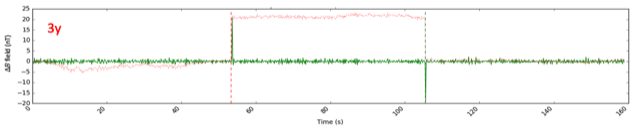
\includegraphics[width=\linewidth, height= 3 cm]{Images/1s1c3y}
        \caption{for 3y and $C_x^-$ }
        \label{fig:1s1c3y}
    \end{subfigure}%
    \begin{subfigure}{.5\linewidth}
        \centering
        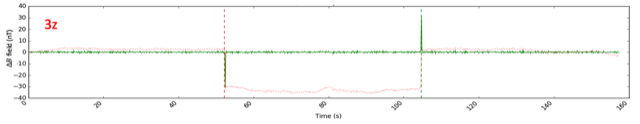
\includegraphics[width=\linewidth, height= 3 cm]{Images/1s1c3z}
        \caption{for 3z and $C_x^-$}
        \label{fig:1s1c3z}
    \end{subfigure}\\[1ex]
    \begin{subfigure}{.5\linewidth}
        \centering
        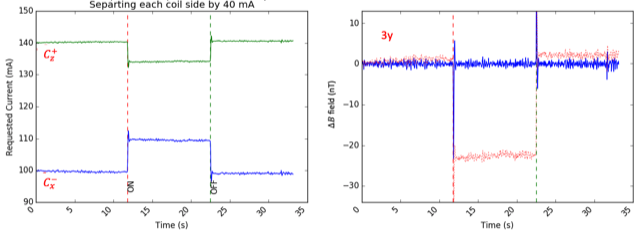
\includegraphics[width=\linewidth, height= 3 cm]{Images/1s2c3yc1c6}
        \caption{for 3y, 3z, $C_x^-$ and $C_z^+$}
        \label{fig:1s2c3yc1c6}
    \end{subfigure}%
        \begin{subfigure}{.5\linewidth}
        \centering
        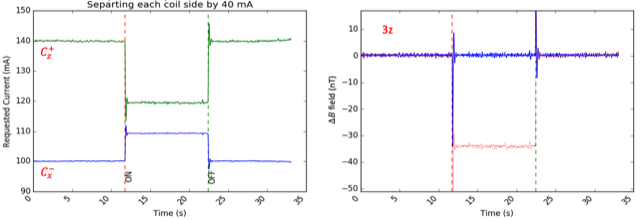
\includegraphics[width=\linewidth, height= 3 cm]{Images/1s2c3zc1c6}
        \caption{for 3y, 3z, $C_x^-$ and $C_z^+$}
        \label{fig:1s2c3zc1c6}
    \end{subfigure}\\[1ex]
    \begin{subfigure}{1\linewidth}
        \centering
        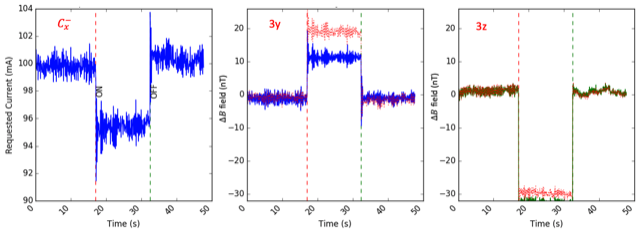
\includegraphics[width=\linewidth, height= 3 cm]{Images/2s1c3y3zc1}
        \caption{for 3y, 3z and $C_x^-$ }
        \label{fig:2s1c3y3zc1}
    \end{subfigure}

    \caption{The compensation effect due to individual coil. Vertical axis in Fig.~\ref{fig:1s1c3y} and in Fig~\ref{fig:1s1c3z} shows the $\Delta$ B found using Eq.~\ref{eq:del_B} over time for two different sensors where the green indicates $\Delta$ B due to compensation and the red indicates $\Delta$ B without compensation. Vertical axis in left of both Fig.~\ref{fig:1s2c3yc1c6} and  Fig.~\ref{fig:1s2c3zc1c6} indicates the coil current that has been sent to coils $C_x^-$ and $C_z^+$ to satblize 3y and 3z as shoen in right of those respectively. Initially both $C_x^-$ and $C_z^+$ were in the same level but for showing them together in the same figure they have been separated by some constant.  Vertical axis in left of Fig.~\ref{fig:2s1c3y3zc1} also indicates the current but only for $C_x^-$. Vertical axis in right of Fig.~\ref{fig:1s2c3yc1c6} and  Fig.~\ref{fig:1s2c3zc1c6} and in middle and right of Fig.~\ref{fig:2s1c3y3zc1} have the same description as in in Fig~\ref{fig:1s1c3z} }
    \label{fig:1d}
\end{figure}

\FloatBarrier
The alternative option has been shown on \textcolor{blue}{7.2.3} of the same study where more sensors than coils with some optimization give better compensation forming a non-square matrix which needs to be inverted for calculating the error using Eq.~\ref{eq:del_I}. The Moore--Penrose pseudoinverse \cite{pseudo} or simply pseudoinverse can be used for the inversion. The pseudoinverse of a matrix can be computed using singular value decompostion (SVD) which is a factorization or diagonalization of a matrix. The matrix can be real or complex square matrix or general rectangular matrix. The SVD~\cite{svd2,svd3} of a real matrix $\bm{M}$ with dimension $m \times n$ is 
\begin{equation}\label{eq:m}
        \bm{M} = \bm{U} \bm{\Sigma} \bm{V^T}
\end{equation}
% where, $\bm{U}\:\epsilon\:\mathbb{R}^{m \times m}$, $\bm{V^*}\:\epsilon\:\mathbb{R}^{n \times n}$ 
where, $\bm{U}$ and $\bm{V}$ are the orthogonal matrices with dimensions $m \times m$ and $n \times n$ respectively and $\bm{V^T}$ is the transpose of $\bm{V}$. $\bm{\Sigma}$ is a real non-negative diagonal matrix with same dimension as  $\bm{M}$ and can be written as

\begin{equation*}
\bm{\Sigma} = \begin{pmatrix} 
\Sigma_{11} & 0 \\
0 & \Sigma_{dd} 
\end{pmatrix}
\end{equation*}
where, $\Sigma_{11},..,\Sigma_{dd}=\text{diag}(\sigma_d)$ with $\Sigma_{11}\gg... \Sigma_{dd}\geq0$ and $d=(1,..,n)$ if $\bm{\Sigma}$ has $m \times n$ dimension and are called singular values of $\bm{M}$  and they are the positive square roots of the non-negative eigenvalues of $\bm{M^T}\bm{M}$.

The pseudoinverse of $\bm{M}$ will be then the inverse of $\bm{U}$, $\bm{\Sigma}$ and $\bm{V^T}$ and can be written as
\begin{equation}\label{eq:psMinv}
    \bm{M^{-1}} = \bm{V \Sigma^{-1} U^T}
\end{equation}
% ${\rm I\!R}$




But the matrix is found to be ill-conditioned which implies that it has got a large condition number which measure the change in the output for a small change in input. The condition number of $\bm{M}$ can be determined from the diagonal matrix $\bm{\Sigma}$ as 
 \begin{equation}\label{eq:cond}
     cond(\bm{M})=\frac{max(\sigma_1)}{min(\sigma_d)}
 \end{equation}
 

The $\Sigma$ for a test $\bm{M}$ has been shown in Fig.~\ref{fig:v} where as discussed earlier except diagonal ones all are zero with the diagonal values are arranged from $\Sigma_{11}$ to $\Sigma_{dd}$ in a decreasing order each having non-negative values. Using the Eq.~\ref{eq:cond}, the condition number of $\bm{M}$=5724/53=108. The minimum condition number of $\bm{M}$ for the prototype is to be 40 and so the $\bm{M^{-1}}$ that calculated using Eq.~\ref{eq:psMinv} is producing unexpected huge currents. 

\fig{Images/v}{width = \textwidth}{Color map of $\Sigma$ for a test $\bm{M}$ found using Python programming language. Horizontal axis indicates the various coils, which are counted using the index $c$. Vertical axis indicates the various sensors, which are counted using the index $s$. Red elements indicate positive values while blue elements indicate near zero values. \label{fig:v}}{short caption}

\FloatBarrier

The problem can visualized from Fig.~\ref{fig:m} where for example X-(1) has negligible sensitivity for 3x which means that particular matrix element (in nT/A) is very small. So, the pseudoinverse of $\bm{M}$ using Eq.~\ref{eq:psMinv} will produce very large element (in A/nT) which means that the amount of current will be huge there which will make the prototype unstable. To minimize the effect, the matrix must be regularized which means that all ill-conditioned places must be replaced  by well-conditioned ones.  Tikhonov regularization~\cite{tikhonov2013numerical,tikhonov_book,svd,svd3} is one of the most commonly used regularization methods which modifies the diagonal elements of $\Sigma^{-1}$ from Eq.~(\ref{eq:psMinv}) that's $\Sigma^{-1}_{dd}$ i.e. $\sigma_d^{-1}$ as

\begin{equation}
    \frac{1}{\sigma_d} \rightarrow \frac{\sigma_d}{\sigma_d^2+\alpha^2} 
\end{equation}
which has been further modified by stating $\alpha=10^r$ in the previous study \cite{bea}) as
\begin{equation}\label{eq:sigma}
    \frac{1}{\sigma_d} \rightarrow \frac{\sigma_d}{\sigma_d^2+(10^r)^2}
\end{equation}

So, the Eq.~(\ref{eq:psMinv}) will be modified due to the modified form of Tikhnov regularization as
\begin{equation}\label{eq:minvR}
    \bm{M^{-1}}(r) = \bm{V}\begin{pmatrix} 
\frac{\sigma_1}{\sigma_1^2+(10^r)^2} & 0 \\
0 & \frac{\sigma_d}{\sigma_d^2+(10^r)^2}
\end{pmatrix} \bm{U^T}
\end{equation}
where, $r$ is called the regularization parameter and  $r \rightarrow - \infty$ will make Eq.~(\ref{eq:minvR}) same as Eq.~(\ref{eq:psMinv}) which is responsible big current fluctuations as described earlier whereas $r \rightarrow + \infty$ results in $\bm{M^{-1}} \rightarrow 0$ i.e. no control.

Generally, $r$ should be within the order of $log(\sigma_{d})$ and the $r$ can be selected using several iterative methods. The obtained $r$ can be directly used in feedback algorithm and PI parameter can be tuned or that can be further changed alongside tuning PI parameters by observing it's effect on current response (see section \ref{sec:r_pi}).


An iterative method has been discussed in  the previous study~\cite{bea} to find $r$. The concept has been applied to the prototype which will be discussed next.

\subsection{Monte Carlo Simulation to Find 'r'}\label{sec:mont}

Here, the simulation model of the previous study~\cite{bea} has been reproduced for the prototype to determine which value of $r$ produce optimal solution for compensation. Starting with relating $r$ with current fluctuation and field fluctuation, the section ends with a suitable value of $r$ to minimize both of the fluctuations.

For the simulation model, a different sets of reasonable random magnetic fields ($B_s^{\text{rand}}$) are generated with center of distribution being 0 and standard deviation 5 nT  based on the horizontal axis of Fig~\ref{fig:dbts} at sensor positions specified by the legends in the figure. The figure is showing the histogram of the difference in magnetic field in nT/s over 24 hours and calcluted as 
\begin{equation}
    \text{Difference in}\;B=B(t+1)-B(t)
\end{equation}
where, the B field has been measured in every 1 second.

\fig{Images/dbts2}{width = \textwidth}{Histogram of the difference in the magnetic field in nT/s indicated by the horizontal axis for different sensor positions specified different colors respectively over 24 hours starting at 1 pm CST on 29 August, 2018 at the prototype site at University of Winnipeg. \label{fig:dbts}}

\FloatBarrier
As the center of the distribution according to Fig.~\ref{fig:dbts} is zero, so using setpoint as zero, according to Eq.~(\ref{eq:del_B}) the drift in the B field will be  
\begin{equation}\label{eq:del_Bs}
    \Delta B_s^{\text{sim}} = 0 - B_s^{\text{rand}}=-B_s^{\text{rand}}
\end{equation}

And thus an array of the current error  as function of $r$ due to the drift caused by $\Delta B_s^{\text{sim}}$ will be calculated using the product of regularized pseudoinverse found using Eq.~(\ref{eq:minvR}) and $\Delta B_s^{\text{sim}}$ which is similar to Eq.~(\ref{eq:del_I})
\begin{equation}\label{eq:del_Is}
    \Delta I_c^{\text{sim}}(r) =\sum_s^{s=1-12} M^{-1}_{cs}(r) \Delta B_s^{\text{sim}}=\sum_s^{s=1-12} M^{-1}_{cs}(r) (-B_s^{\text{rand}})
\end{equation}

Also the to get the overall response from the array of the current, the root mean square (RMS) of $\Delta I_c^{\text{sim}}(r)$ found using Eq.~(\ref{eq:del_Is}) will be calculated as
\begin{equation}
     \Delta I_{\text{RMS}}^{\text{sim}}(r)= \sqrt{\sum_c^{c=1-6} \frac{1}{c}(\Delta I_c^{\text{sim}}(r))^2}
\end{equation}
As, $\Delta I_c^{\text{sim}}(r)$ depends on both $r$ and $B_s^{\text{rand}}$, so to see the effect of current on the perturbation, $\Delta I_c^{\text{sim}}(r)$ and thus $ \Delta I_{\text{RMS}}^{\text{sim}}(r)$  has been calculated for different sets of $B_s^{\text{rand}}$ as a function of $r$. In Fig.~\ref{fig:Isim}, $ \Delta I_{\text{RMS}}^{\text{sim}}(r)$ as indicated by vertical axis over $r$ as indicated by horizontal axis has been shown for 30 different sets of $B_s^{\text{rand}}$. The distribution $B_s^{\text{rand}}$ is randomly chosen with center of distribution and standard deviation is discussed earlier. It is noticeable that with increase of $r$, the current fluctuations $\Delta I_c^{\text{simRMS}}$ are vanished as expected according to Eq.~(\ref{eq:minvR}).

\fig{Images/6c_I}{width = \textwidth,height =9.5cm}{The effect of $r$ on the current fluctuations due to 30 different sets of $B_s^{\text{rand}}$ with the distribution described in the text. Horizontal axis represents different valu of $r$ while vertical axis is showing $\Delta I_c^{\text{simRMS}}$ found due to different sets of $B_s^{\text{rand}}$. \label{fig:Isim}}{short caption}

\FloatBarrier
The field produced by $ \Delta I_c^{\text{sim}}$ can be calculated using Eq.~(\ref{eq:B_coils}). Thus the total field will be the superposition of $B_s^{\text{rand}}$ and the field produced by $ \Delta I_c^{\text{sim}}(r)$ and is given by
\begin{equation}\label{eq:B_coils-sim}
    B_s^{\text{sim}}(r) =\sum_c^{c=1-6} M_{sc} \Delta I_c^{\text{sim}}(r) + B_s^{\text{rand}}
\end{equation}

For a fully compensated system, the field produced by $ \Delta I_c^{\text{sim}}$ will be equal to $- B_s^{\text{rand}}$ which in turns make the $B_s^{\text{sim}}(r)$ according to Eq.~(\ref{eq:B_coils-sim}) as zero as it should be because the setpoint has been considered to be zero. Now, to see the effect of $ \Delta I_c^{\text{sim}}(r)$ on the $B_s^{\text{rand}}$ i.e. how much compensation has been possible due to the field produced by $ \Delta I_c^{\text{sim}}(r)$,  the ratio of RMS of $B_s^{\text{sim}}(r)$ to the RMS of $B_s^{\text{rand}}$ has been calculated as
\begin{equation}\label{eq:fluc}
    F(r)=\frac{\sqrt{\sum_s \frac{1}{s}(B_s^{\text{sim}}(r))^2}}{\sqrt{\sum_s \frac{1}{s}(B_s^{\text{rand}}(r))^2}}
\end{equation}
So, for a fully compensated system as discussed earlier, the numerator of Eq.~(\ref{eq:fluc}) will be zero which makes $F(r)$ to be zero. So, for a fully compensated system $F(r)$ should be zero. The effect of $r$ on the compensation due to the field produced by $ \Delta I_c^{\text{sim}}(r)$ to counteract $B_s^{\text{rand}}$ is shown in Fig.~\ref{fig:fluc-sim} for same sets of $B_s^{\text{rand}}$ as stated earlier. It is seen that with the increase of $r$, the field produced due to $\Delta I_c^{\text{sim}}$ to compensate $B_s^{\text{rand}}$  are increasing i.e. more field fluctuations. It is also noticeable that the systems can not be fully compensated due to the field produced by $ \Delta I_c^{\text{sim}}(r)$ as $F(r)$ never goes to zero. The lowest $F(r)$ goes to 0.45. That means the highest compensation due to the field produced by  $\Delta I_c^{\text{sim}}$ to counteract $B_s^{\text{rand}}$ is (1-0.45$\times$100)$\%=$55$\%$.

\fig{Images/6c_f}{width = \textwidth,height =9.5cm}{The effect of $r$ on horizontal axis on the compensation due to the field produced by $ \Delta I_c^{\text{sim}}(r)$ to counteract $B_s^{\text{rand}}$ indicated by $F(r)$ on vertical axis. The different curves indicate 30 different sets of $B_s^{\text{rand}}$ with the distribution describes earlier. \label{fig:fluc-sim}}{short caption}

\FloatBarrier
It is seen from the Fig.~\ref{fig:Isim} and Fig.~\ref{fig:fluc-sim} that with the increase of $r$, current fluctuations are decreasing but field fluctuations are increasing respectively. So, a compromise between them has to be determined to figure out the value of $r$ which will optimally response for less field and current fluctuations.  That is, small current fluctuations ($r \rightarrow + \infty$) has to be traded off against small magnetic field fluctuations ($r \rightarrow - \infty$). For that, first $\Delta I_{\text{RMS}}^{\text{sim}}(r)$ and $F(r)$ were normalized as

\begin{equation}\label{eq:Inorm}
    \overline{\Delta I_{\text{RMS}}^{\text{sim}}}(r)=\frac{\Delta I_{\text{RMS}}^{\text{sim}}(r)}{\Delta I_{\text{RMS}}^{\text{sim}}(r\rightarrow - \infty)}
\end{equation}
\begin{equation}\label{eq:flucNorm}
    \overline{F}(r)=\frac{F(r)- F(r\rightarrow - \infty)}{F(r\rightarrow \infty)- F(r\rightarrow - \infty)}
\end{equation}

Now, the value of $r$ for which the normalized value of $\Delta I_{\text{RMS}}^{\text{sim}}(r)$ and $F(r)$  as found using Eq.~(\ref{eq:Inorm}) and Eq.~(\ref{eq:flucNorm}) respectively produce $0.5$ has been stored for for same previously stated set of $B_s^{\text{rand}}$ and the stored $r$ are then averaged to finally get the optimized $r$. 

The effect of $r$ on $\overline{\Delta I_{\text{RMS}}^{\text{sim}}}$ and $\overline{F}$ are shown in Fig.~\ref{fig:I-fluc} where with increase $r$, $\overline{\Delta I_{\text{RMS}}^{\text{sim}}}$ decreases and $\overline{F}$ increases as expected from the discussion earlier. The optimized $r$ for the process described above has been found to be 2.87.

\fig{Images/6c_I-fluc2}{width = \textwidth,height=9cm}{The effect of $r$ indicated by horizonatl axis on $\overline{\Delta I_{\text{RMS}}^{\text{sim}}}$ indicated by left vertical axis and $\overline{F}$ indicated by right vertical. The different curves on both vertical axes indicate 30 different sets of $B_s^{\text{rand}}$ with the distribution describes earlier. The red lin indicates the 0.5 level in the figure.  \label{fig:I-fluc}}{short caption}

\FloatBarrier

So, the simulation model to find $r$ gives the insight about the effect of $r$ on current and filed fluctuations and also produce a suitable value of $r$ to compromised both fluctuations. Agter having $r$, its time to tune the PI parameter to get the current as given in Eq.~(\ref{eq:I}) which will be discussed next.

\section{Tuning of PI Parameter}\label{sec:tune}
This section is about tuning the Proportional (P) gain i.e. $k_c^p$ and Integral (I) reset i.e. $k_c^i$ term which are needed to calculate the required current as in Eq.~(\ref{eq:I}) to compensate the drift in magnetic fields producing due to the fluxgate sensors at various positions within the prototype.



According to the type of system and the way the control loop for a particular system has been chosen, the P and I can be tuned using various methods~\cite{tuning}. For the prototype, as we have a closed loop system with desired setpoint to meet, the best possible tuning method is Ziegler-Nichols closed tuning method~\cite{tuning_ZN}. Here, the tuning will be described by applying to the prototype. So, the variable in our case are the currents in all the six coils that generate the field to counter balance the drift in magnetic signals. So, for tuning, first the I term or $k_c^i$ value in Eq.~(\ref{eq:I}) is set to zero and gradually increases the P term or $k_c^p$ value until the currents in the different coils start oscillating. The $k_c^p$ value for which the current in the coils start oscillating is noted as ultimate gain ($G_{u}$) and the period for that is noted as ultimate oscillation period ($T_u$). Now the the value of $k_c^p$ and $k_c^i$ are chosen based on the PI on the Table~\ref{table:tuning} where the formula to find them are given in terms of only P controller and PI controller~\cite{tuning_formula}. 

\begin{table} [htb!]
    \centering
    \begin{tabular} { |c|c|c|c|c|c|} 
        \hline
        Controller & Gain (P or $k_c^p$ ) & Reset (I or $k_c^i$)\\
        \hline\hline
         P & 0.5 $G_u$ & 0 \\ 
        \hline
         PI & 0.45 $G_u$ & $\left(\frac{\text{0.54} G_u}{T_u}\right)\Delta t$ \\ 
        \hline
    \end{tabular}
    % \vspace{4mm}
    \caption{Ziegler-Nichols tuning method for P and PI controller. }\label{table:tuning}
\end{table}

\FloatBarrier
Here, the formula for finding $k_c^i$ has been derived from the original formula which is $T_i=T_u/1.2$ with $k_c^i=(k_c^p/T_i)\Delta t$ and so
\begin{equation}
    k_c^i=\left(\frac{k_c^p}{T_u/1.2}\right)\Delta t=\left(\frac{1.2\times0.45 G_u}{T_u}\right)\Delta t=\left(\frac{0.54 G_u}{T_u}\right)\Delta t
\end{equation}
where, $\Delta t$ is the time difference between two consecutive feedback loop.
\doublefig{Images/p97}{width =\textwidth,height=8cm}{at $k_c^p$=0.97. \label{fig:tuningNmod}}{Images/p97mod}{width = \textwidth,height=8cm}{$k_c^p$=0.97 with zoomed $C_y^-$.\label{fig:tuningMod}}{{The current behaviour in all six coils with $k_c^p$ =0.97 and $k_c^i$=0. Vertical axes represent the currents in all six coils having different colors. The 'ON' and 'OFF' vertical dashed lines indicate the time of the perturbation coil being turned 'ON' and 'OFF' respectively. Both the figures are same except the current in $C_z^+$ coil has been zoomed in left figure.  } \label{fig:tuning}}


The Fig.~\ref{fig:tuning} is showing the tuning for the prototype. At $k_c^p$=0.97 and $k_c^i$=0, the current in the coils are start oscillating to an extent as shown in Fig.~\ref{fig:tuningNmod}. So, the $k_c^p$=0.97 is the ultimate gain $G_u$. Now, for that $G_u$ the ultimate period $T_u$ has to be obtained which is done by zooming the current in coil $C_y^-$ as shown in Fig.~\ref{fig:tuningMod} and is found to be $T_u$=0.3s. Now according to Table~\ref{table:tuning}

\begin{equation}
    k_c^p=0.45\times0.97=0.44\;\;\text{and}\;\; k_c^i=0.54\times0.97/0.3=1.75
\end{equation}


They can be further tuned for the individual coil currents according to necessity. More about PI tuning will be discussed in the next chapter with compensation results. Next, a simulation model will be discussed to quantify the prototype.

% Moreover, to double check, the experimentally obtained $\bm{M}$ has been compared with a simulation done using finite element analysis (FEA) via Opera 3D software as shown in Fig.\ref{fig:Mdiff}.


%  \fig{Images/Mdiff}{width =  \textwidth}{Comparison of Experimental M with Simulation \label{fig:Mdiff}}
 
 
% 

% Fig.\ref{fig:bt} shows the compensation over time with applied perturbation. \newpage
\FloatBarrier
\section{Simulation of Prototype Integrating Feedback Algorithm}

To show the experimental results make sense, a simulation has been. This section starts with describing the simulation software for making the experimental setup geometry and extracting the magnetic field values in that geometry and then move forward to all the simulations made to run a fully functional PI simulation. For, data analysis, sorting  and modifying the data and also running the PI control algorithm the Python programming language has been used alongside the simulation software. The complete simulation is made of three different simulations. 

\begin{itemize}
    \item Simulation of Matrix M
    \item Simulation of Magnetic Field Distribution
    \item Simulation of PI Control
\end{itemize}
In the following  all of the above simulations  will be discussed in detail starting with the simulation software itself. The section ends with comparing the simulation results with the experimental ones.

\subsection{About Simulation Software}
Here, the simulation software has been discussed in detail. Mainly, the focus is on the the module of the software that we have used .

OPERA 3D Finite Element Analysis~(FEA)~\cite{opera} simulation software has been used for making the geometry of the prototype and extracting the magnetic field values along with applying current in the coils including the perturbation one. OPERA is a multi-physics software package which allows coupled simulations including the ability to couple a Static Module simulation with a thermal simulation or a stress simulation, for example to calculate the stress due to electromagnetic forces. We have used the Opera Static Electromagnetics Module which computes magnetostatic and electrostatic fields or direct current (DC) flow in three dimensions. The module solves Maxwell$'$s equations for the static case in a discretized model using FEA. The module automatically switches to the part containing magnetic spruces in case of magnetostatics. In this module, the properties of the magnetic materials can be specified as required i.e. linear, non-linear, isotropic, anisotropic, laminated or permanent magnet. For calculating magnetic fields from coils, the module uses Biot-Savart integral equation. To calculate the potential at each node of the mesh, OPERA uses an iterative solution technique which is memory-efficient and computationally fast.

In the upcoming Sections, the geometry that has been built will be discussed along with all the steps done to finally make a PI control simulation


\subsection{Experimental Setup in OPERA 3D FEA}

Here, the process to build the prototype geometry in the OPERA has been discussed both with outermost layer of passive shielding and without the shield.

In Section~\ref{sec:shield}, the mu-metal shields with the dimension of each of the shield layer have been discussed. Using those information the shield geometry has first been written in a file format known as 'comi' file which acts as command language to run the OPERA FEA simulation software. And then racetracks have been used to draw the coils round the shield including the perturbation one and the drawing command has also been written in the same 'comi' file. The coils properties have been taken from Section~\ref{sec:cube} where the dimension of the coils including the perturbation coil have been discussed. Another 'comi' file has been written where the mu-metal information has been ignored. The two 'comi' files while running individually in OPERA produce prototype geometry which has been shown with outermost passive shielding layer in Fig. \ref{fig:shield_opera} and that without any passive shielding layer in Fig. \ref{fig:noShield_opera} respectively. The dots in Fig. \ref{fig:noShield_opera} represents some fluxgate positions which can be anything with the labelling is discussed in Table~\ref{table:index}.

\doublefig{Images/shield}{width =\textwidth,height =8cm}{with passive shielding layers. \label{fig:shield_opera}}{Images/noShield}{width = \textwidth,height =8cm}{without outermost passive shielding layer.\label{fig:noShield_opera}}{{Prototype setup in OPERA simulation software with outermost passive shielding layer (left)  and without any passive shielding layer (right). The coil in the far side in both of the figures is the perturbation coil. The shield dimensions and properties are given in Section~\ref{sec:shield}  and that of coils are given in Section~\ref{sec:cube}. The direction of each of the three axis has been shown in the right figure.} \label{fig:opera_setup}}

\FloatBarrier

After getting the prototype geometry in OPERA, the next is to discuss the simulation made to calculate the matrix elements and thus produce the matrix $\bm{M}$.

\subsection{Simulation of Matrix M}\label{sec:mSim}

Here, matrix elements $M_{sc}$ that are measured in Section~\ref{sec:m} to produce $\bm{M}$ will be reproduced in this simulation with exactly the same location of the sensor positions and coils. 

 First, a 'comi' file is written where the magnetic field contribution due to environment is set to zero as  matrix elements $M_{sc}$ relate the coils current to the field produced by the coils current (see Eq.~(\ref{eq:B_coils})). Now as matrix elements $M_{sc}$ are in the unit of nT/A, in the same 'comi' file current for the all the six coils have set to 1A which makes the Eq.~(\ref{eq:B_coils}) as

\begin{equation}\label{eq:B_coils_1A}
    B_s(\text{coils})=\sum_c^{c=1-6} M_{sc}
\end{equation}
where, $n$=1.

Now the 'comi' file for the above setup will interact with the 'comi' file of the prototype geometry and then by using the solver of OPERA, $B_s(\text{coils})$ i.e. $M_{sc}$ elements will be calculated.  The best thing about simulating in this setting is that the OPERA has calculated the $M_{sc}$ elements for the whole volume of the prototype geometry which can be easily exported in a 'csv' file by running a simple 'comi' file for volume extraction. Thus the $M_{sc}$ elements of the whole prototype geometry have been stored in a 'csv' file in T/A. Then, a code has been written in the Python programming language to clean, modify and sort the data of that 'csv' file and convert the data in nT/A and  provide the co-ordinates of the points from where the magnetic field values i.e.  $M_{sc}$ elements (see Eq.~(\ref{eq:B_coils_1A})) are determined. For the comparison with the experimental $\bm{M}(\text{exp})$, the simulation $\bm{M}(\text{sim})$ has been made by choosing co-ordinates of the point as same as the sensor positions in the experiment and then the absolute differences of the  $M_{sc}$ elements ( $M_{\text{diff}}^{\text{abs}}$ ) of them are calculated as

\begin{equation}
    M_{\text{diff}}^{\text{abs}}=\frac{\text{abs}(M_{sc}^{\text{abs}}(\text{exp})-M_{sc}^{\text{abs}}(\text{sim}))}{1000}
\end{equation}
where, $M_{sc}^{\text{abs}}(\text{exp})$ and $M_{sc}^{\text{abs}}(\text{sim})$ indicate the absolute values of $M_{sc}$ elements both in experiment and simulation respectively which are in nT/A. For better visualization the differences have been divided by 1000 to get $M_{\text{diff}}^{\text{abs}}$ in $\mu$T/A. 
% And the current in the coils are related to the magnetic filed with those $M_{sc}$ elements as given in Eq.~(\ref{eq:B_coils}). It is very easy to extract magnetic field information by providing the co-ordinates vale in OPERA. In addition to the field produced by the coil currents, there is also  values of $M_{sc}$. That means, setting current, I=1 A and offset =0 in all six coil will produce 
% \fig{Images/noShield}{width =\textwidth,height=14 cm}{Prototype setup in OPERA simulation software without passive shielding layers. \label{fig:noShield_opera}}
The comparison in terms of $M_{\text{diff}}^{\text{abs}}$ has been shown in Fig. \ref{fig:Mdiff}. It is seen that most of the $M_{\text{diff}}^{\text{abs}}$ differences are very small that means the simulation results match the experimental one. It is also noticeable that in some places, the $M_{\text{diff}}^{\text{abs}}$ are around 1 $\mu$T/A difference which is normal as its not possible to exactly pinpoint the locations both in experiment and simulation and also the simulation runs in ideal conditions where the experiment suffers from the condition of its surrounding. But overall the result is quite satisfactory.

\fig{Images/Mdiff_37}{width = \textwidth}{The absolute differences between the  $M_{sc}$ elements experiment with that of simulation in $\mu$T/A. Horizontal axis indicates the various sensors, which are counted using the index $s$. Vertical axis indicates the various coils, which are counted using the index $c$.  Red elements indicate positive values while blue elements indicate near zero values. \label{fig:Mdiff}}{short caption}

\FloatBarrier
So, we have made simulation which can produce $M_{sc}$ elements for any number of the sensors placed in the prototype geometry. This will be a huge tool for the future students who are limited by sensor position and placing them correctly in their system to study in detail about the effect of $\bm{M}$ for any set of sensors.


\subsection{Simulation of Magnetic Field Distribution}\label{sec:pSim}

We have already got the prototype geometry  from the above discussion. Here, the magnetic field distribution without any current in the coils that is $B_s(\text{setpoint})$ and due to the current in the perturbation coil that is $B_s(\text{measure})$ will be determined. From those the drift in the signal will be determined using Eq.~(\ref{eq:del_B}) and lastly how the perturbation affects the current in all six coil sides will be discussed. 

\subsubsection{Simulation of B (setpoint)}
 
Here, the magnetic field distribution without any current in the coils that is $B_s(\text{setpoint})$ will be determined by simulating the prototype in OPERA.

First, a 'comi' file is written with setting the currents in all the coils including the perturbation one to zero. In this case, the magnetic field values of the environment surrounding the prototype are set according to Table~\ref{table:Benvironment}. Then the 'comi' file interact with the 'comi' file of the prototype geometry to run combinely in OPERA for simulation. After finishing the simulation the volume extraction 'comi' file will be run to export the magnetic field values of the whole prototype geometry into a 'csv' file. Finally, the data on that 'csv' file is cleaned, modified and the magnetic field values within the prototype are generated by providing the co-ordinates of the specified positions via the Python programming language which are act as $B_s(\text{setpoint})$.

\subsubsection{Simulation of B (measure)}

Here, the magnetic field distribution for current in the perturbation coil that is $B_s(\text{measure})$ will be determined by simulating the prototype in OPERA.


To simulate $B_s(\text{measure})$ for a particular perturbation simialr steps have been taken as above except in this case, the current in the perturbation coil has been set to 770 mA. The reason of choosing 770 mA current in the perturbation coil is that in the experiment, 10 mA current has been provided to the perturbation coil with 77 no of turns. So, with this setting again a 'comi' file has been made which interacts with the 'comi' file of the prototype geometry to run combinely in OPERA for simulation. After finishing the simulation the volume extraction 'comi' file will be run to export the magnetic field values of the whole prototype geometry into a 'csv' file. Finally, the data on that 'csv' file is cleaned, modified and the magnetic field values within the prototype are generated by providing the co-ordinates of the specified positions via the Python programming language which are act as $B_s(\text{measure})$.



For comparing the simulation result with experimental one, the effect of the perturbation has been found in terms of change in the coil currents in all six coils both in simulation and experiment. For the simulation, in the above, $B_s(\text{setpoint})$ and $B_s(\text{measure})$ have been determined by choosing co-ordinates of the points as same as the sensor positions in the experiment form which the drift in the signal i.e. $\Delta B_s$ have been determined using Eq.~(\ref{eq:del_B}). Finally, the change in the coils current i.e. the errors in the coils have been determined by multiplying $\Delta B_s$ with regularized pseudo-inverse of $\bm{M(\text{sim})}$ obtained from Section~\ref{sec:mSim} (see Eq.~(\ref{eq:del_I}) and Section~\ref{sec:inv}). For experiment the drifts in the fluxgate signals are determined by applying 10 mA in the perturbation  coil and then find $\Delta B_s$ using Eq.~(\ref{eq:del_B}) and eventually find the change in coil currents in the same way as done for the simulation. The change in current in all six coil sides found due to experiment and simulation are given in Table~\ref{table:currentChange} where the simulation results are quite similar to the experimental ones for all six coils sides.

\begin{table} [htb!]
    \centering
    \begin{tabular} { |c|c|c|c|c|c|} 
        \hline
        Coils & \makecell{Chage in Current (mA)\\Experiment} & \makecell{Chage in Current (mA)\\Simulation}\\
        \hline\hline
        $C_x^-$ & -26 & -32 \\ 
        \hline
        $C_x^+$ & 22 & 20 \\
        \hline
        $C_y^-$ & -30 & -24 \\
        \hline
        $C_y^+$ & 24 & 17 \\
        \hline
        $C_z^-$ & -14 & -13 \\
        \hline
        $C_z^+$ & 54 & 46 \\
        \hline

    \end{tabular}
    % \vspace{4mm}
    \caption{Comparison of change in current in different coil sides at the time of applying perturbation both in experiment and simulation.}\label{table:currentChange}
\end{table}

\FloatBarrier
In the above, simulation has been made via OPERA to find $B_s(\text{setpoint})$ and $B_s(\text{measure})$. For the purpose of comparison using those values the change in current in all six coil sides have been found and matched with experimental results. In the upcoming Section the results obtained due to various simulation will be used to make a fully functional PI simualtion.
% The values obtained due to this have been compared with the values due to experimental setup and the results are similar as shown in Fig. \ref{fig:noShield_cSim}.

% \fig{Images/cSim}{width =\textwidth, height=14cm}{Comparison of change in current in different Coil sides at the time of applying perturbation both in experiment and simulation. \label{fig:noShield_cSim}}


\subsection{PI Simulation}
Here, the simulation results from the above discussed Sections will be integrated to a new simulation to run PI control algorithm in time.

From the previous Sections of the simulation, there are already values of $B_s(\text{setpoint})$, $B_s(\text{measure})$ and $\bm{M(\text{sim})}$ which will give the errors following the Eq.~(\ref{eq:del_B}), concept in Section~\ref{sec:inv} and Eq.~(\ref{eq:del_I}). Then, the value of $k_c^p$ and $k_c^i$ has been obatined by following the concept of PI tuning as discussed in Section~\ref{sec:tune}. After getting the tuned value of $k_c^p$ and $k_c^i$, the new current that should be fed to the coils for compensating the magnetic field drift is calculated using Eq.~(\ref{eq:I}). The same process have been repeated for a time duration. Thus, a PI simulation in time has been made. 

The magnetic field compensation due to PI feedback loop has been shown in terms of experiment in Fig.~\ref{fig:pi_exp_all} and that of simulation in Fig.~\ref{fig:pi_sim_all}, where in the top rows all the reds indicate the compensation results while the colors represent the uncompensated magnetic fields in $x$, $y$ and $z$ axis respectively and the bottom row with different colors  indicates only the compensated magnetic fields in $x$, $y$ and $z$ axis respectively. The uncompensated magnetic field is the magnetic field without the compensation effect and predicted by
\begin{equation}\label{eq:Buncomp}
    B_s^n(\text{uncompensated})=B_s^n(\text{measured})- B_s^n(\text{coils})
\end{equation}
where, $B_s^n(\text{measured})$ is the actual measurement from coming the fluxgate sensors in experiment or determined using simulation (see Section~\ref{sec:pSim}) with $n$=(1,...N) is the no of measurements taken and $B_s^n(coils)$ is determined using Eq.~(\ref{eq:B_coils}). The results from experiment and simulation are quite simialr.

\FloatBarrier
\doublefig{Images/pi_exp_all}{width =\textwidth, height=10cm}{Experiment\label{fig:pi_exp_all}}{Images/pi_sim_all}{width = \textwidth,height=10cm}{Simulation\label{fig:pi_sim_all}}{{PI active magnetic field compensation results by both Experiment (a) and Simulation (b). Vertical axis represents the $\Delta B_s$ (see Eq~(\ref{eq:del_B})) and the horizontal axis represent the time. All the colors has been discussed in the text. The 'ON' and 'OFF' vertical dashed lines indicate the time of the perturbation coil being turned 'ON' and 'OFF' respectively. } \label{fig:pi_ExpSim_all}}

\FloatBarrier




% Again, the same result has been shown by separating $x$, $y$ and $z$ respectively in Fig. \ref{fig:pi_exp} obtained by experiment and in Fig. \ref{fig:pi_sim} due to simulation.

% \fig{Images/pi_exp}{width =\textwidth,height=14cm}{PI Active Magnetic Field Compensation Results in $x$, $y$ and $z$ axis by both Experiment. \label{fig:pi_exp}}

% \fig{Images/pi_sim}{width =\textwidth,height=14cm}{PI Active Magnetic Field Compensation Results in $x$, $y$ and $z$ axis by both Simulation. \label{fig:pi_sim}}


Simulation of a certain system integrating feedback algorithm is a unique work that has not been still published in any thesis related to active compensation.

\section{Metrics\label{sec:metrics}}
For every system, there are some metrics, based upon whom the system will be justified. The success of the prototype has been claimed similarly. Mainly, four areas have been looked into as derived from the previous studies \cite{bea,lins,rawlik}. They are discussed in the following subsections.

\subsection{Condition Number and Regularization Parameter}
The condition number of a matrix and its relation to the regularization parameter has already been discussed in Section~\ref{sec:inv}. The main aim is to make the prototype well-conditioned by determining the best compromise between current and field fluctuations which will lead us to the optimized $r$. It has been also explored to determine whether the optimized $r$ is giving the best result or not. If not, additional parameters have been tuned to get the best possible result.

\subsection{Magnetic and Current Fluctuation Reduction}

Active magnetic field compensation come into play in the first place to make the surrounding magnetic fluctuations as minimum as possible. So, prototype response for magnetic fluctuations has been studied in terms of its capabilities as reduction or amplification. As the main concern is about the experiment which will be carried inside the passive shielding, the response has been specially studied on the central sensors. Some of the responses has been shown in Fig. \ref{fig:bt_mod} where the red indicates what is the fluctuation looks like without the compensation and the colors indicate the fluctuation levels after compensation. Moreover, the last one named 'center-Z' predicts the fluctuation in the center of the prototype in $z$ axis without actually being in the feedback loop and there is also improvement in terms of fluctuation.

\fig{Images/bt-mod}{width =\textwidth,height=10cm}{Magnetic field reductions from some of the sensor positions closer to the perturbation coil. Vertical axis represents the $\Delta B_s$ (see Eq~(\ref{eq:del_B})) and the horizontal axis represent the time. All the colors has been discussed in the text. The 'ON' and 'OFF' vertical dashed lines indicate the time of the perturbation coil being turned 'ON' and 'OFF' respectively. \label{fig:bt_mod}}{short caption}

\subsection{PI Behavior to Stimuli}
 Tuning is one of the main factor of PI control feedback algorithm. After going through all the steps, it needs to have a suitable value of PI parameters which can be obtained by tuning the prototype as discussed in section \ref{sec:tune}. Moreover, PI behavior has been also monitored for step response in the perturb electromagnet coil.
 
 \subsection{Allan Deviations and Shielding Factor}
 
Allan standard deviation \cite{allan} is usually applied to the time series to determine the time stability in clocks, amplifiers and oscillators. The same concept can be applied to find the magnetic field stability in time~\cite{bea} as
\begin{equation}\label{eq:adev}
    \sigma_{Adev} (\tau)=\sqrt{\frac{1}{2(N-1)}\sum_{l=1}^{N-1} \left(B_{l+1}(\tau)-B_l(\tau)\right)^2}
\end{equation}
where, $B_l(\tau)$ is the average magnetic field for a sub sample $l$ over integration time $\tau$ and $\tau = \frac{T}{N}$ with $T$ is the total measurement time and $N$ is total number of sub samples. The largest integration time for total measurement time $T$ is $\tau_{\text{max}}=T/2$ and for that the total number of sub sample is $N = \frac{T}{\tau_{\text{max}}}=\frac{T}{T/2}=2$. So, $\sigma_{Adev}(\tau_{\text{max}})$ is negligible since there is only one difference value of sub sample as seen by Eq.~(\ref{eq:adev}).

The Allan deviation of $B_s(\text{measured})$ and $B_s(\text{uncompensated})$ has been shown in the upper part of Fig.~\ref{fig:sf_mod}. $B_s(\text{uncompensated})$ can be predicted using Eq.~(\ref{eq:Buncomp}). The red colors in the upper part of Fig.~\ref{fig:sf_mod} indicates the Allan deviation of $B_s(\text{measured})$ and the colors other than red indicate the  Allan deviation of $B_s(\text{uncompensated})$ in $x$, $y$ and $z$ axis. With increase of integration time $\tau$, the Allan deviation of $B_s(\text{measured})$ is less than the  Allan deviation of $B_s(\text{uncompensated})$ which indicates that the magnetic field is less fluctuated i.e. more stable during compensation than without compensation in time. 
\fig{Images/sf_mod}{width =\textwidth,height=12cm}{The Allan deviation (top) and shielding factor (bottom) for signals from some fluxgate sensors. Top vertical axis indicates the Allan deviation while bottom indicates shielding factor. Horizontal axis indicates the integration time. The different colors in top and bottom have been discussed in text.  \label{fig:sf_mod}}{short caption}

\FloatBarrier

Moreover, to determine the factor by which the magnetic field is more stable in compensation than uncompensated at a given $\tau$, the shielding factor~\cite{bea} has been calculated as
\begin{equation}\label{eq:sf}
    \text{sf} (\tau)=\frac{\sigma_{\text{Adev}}^{\text{uncompensated}}(\tau)}{\sigma_{\text{Adev}}^{\text{measured}}(\tau)}
\end{equation}
So, the shielding factor in any of the fluxgate sensorat a given $\tau$  $>$ 1 indicates that the magnetic field is more stable on compensation than uncompensated on that fluxgate sensor on that $\tau$. Shielding factor is a vital factor to observe the long term stability under no stimulus condition. The shielding factors due to some of the fluxgate sensors have been shown in the lower part of Fig. \ref{fig:sf_mod}. The different colors indicate the  shielding factor in $x$, $y$ and $z$ axis. The shielding factors are found to be always $>$ 1 except at the beginning as the value lower than optimized $r$ has been used for better current response time which introduces some fluctuations as explained in section \ref{sec:r_pi}.
 

%\fig{Images/sf}{width = 0.5 \textwidth}{Allan Deviation and Shielding Factor \label{fig:sf}}
 
 
 